\subsection{Ca sử dụng thao tác trên ảnh}

\vspace{0.5cm}

\noindent 
\begin{tabularx}{\linewidth}{| l | X |} 
\hline 
\textbf{Mô tả} & Người dùng thao tác với ảnh trong thư viện: yêu thích, chỉnh sửa caption, tải ảnh xuống và xóa ảnh. \\
\hline 
\textbf{Luồng cơ bản} & 1. Người dùng chọn ảnh muốn thao tác tron thư viện. \newline
                       2. Hệ thống hiển thị ảnh ở chế độ toàn màn hình cùng thanh công cụ.\newline
                       3. Người dùng bấm nút yêu thích ảnh. \newline
                       4. Hệ thống đánh dấu ảnh là yêu thích và cập nhật giao diện. \newline
                       5. Người dùng bấm nút chỉnh sửa caption ảnh. \newline
                       6. Hệ thống hiển thị form chỉnh sửa caption ảnh. \newline
                       7. Người dùng nhập caption mới và bấm nút lưu. \newline
                       8. Hệ thống cập nhật caption ảnh và cập nhật lại giao diện. \newline
                       9. Người dùng bấm nút tải ảnh xuống. \newline
                       10. Hệ thống lưu ảnh vào máy người dùng và hiển thị thông báo thành công. \newline
                       11. Người dùng bấm nút xóa ảnh. \newline
                       12. Hệ thống xóa ảnh trong thư viện, hiển thị thông báo thành công và hiển thị ảnh tiếp theo. \\
\hline 
\textbf{Luồng thay thế} &
                        - Người dùng không nhập caption / caption ảnh không thay đổi so với caption cũ \\ 
\hline
\textbf{Tiền điều kiện} & - Người dùng đã đăng nhập vào hệ thống. \newline
                           - Người dùng đã có ảnh trong thư viện. \\
\hline
\textbf{Hậu điều kiện} & - Hệ thống cập nhật các thông tin của ảnh được update: yêu thích, caption, ... \\
\hline 
\textbf{Yêu cầu phi chức năng} & Hệ thống xử lý mỗi thao tác không quá 1s. \\
\hline 
\end{tabularx}

\vspace{0.8cm}

\noindent 
\begin{tabular}{| c | c |}
    \hline
    \textbf{Biểu đồ hoạt động} & \textbf{Quan hệ} \\ 
    \hline
    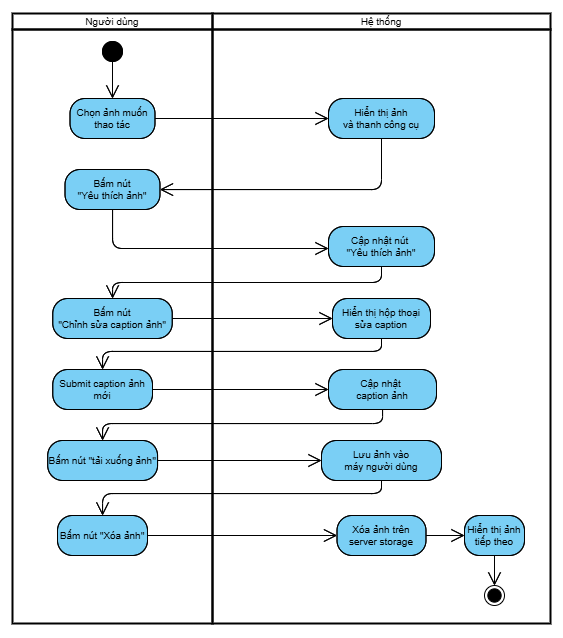
\includegraphics[width=0.6\linewidth]{figures/c3/3-3-6-activity-diagram.png} 
    &  
    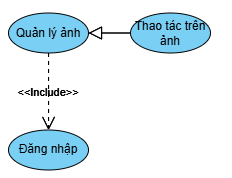
\includegraphics[width=0.35\linewidth]{figures/c3/3-3-6-relationship.png} \\ 
    \hline
\end{tabular}

\begin{figure}[H]
    \centering  
    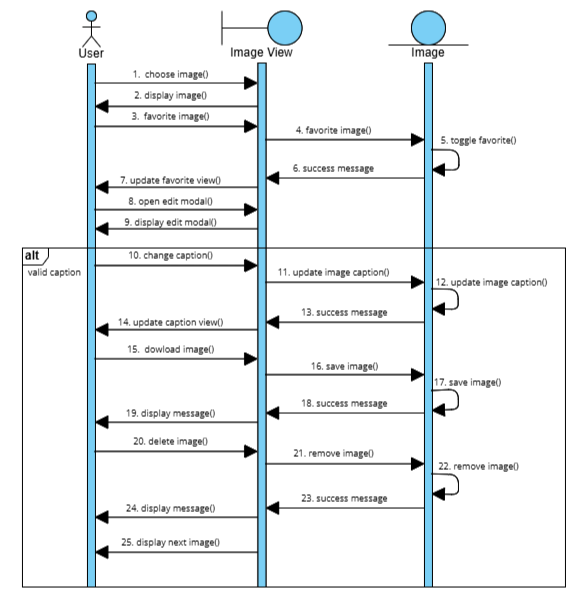
\includegraphics[width=1\textwidth]{figures/c3/3-3-6-sequence-diagram.png}
    \caption{Biểu đồ tuần tự ca sử dụng thao tác trên ảnh.}
    \label{fig:3-3-6-sequence-diagram}
\end{figure}
